\section{Introduction}
Semantic Role Labeling (SRL) is a task in Natural Language Processing (NLP) which aims to automatically assign semantic roles to each argument for each predicate in a given input sentence. As for a brief definition, given an input sentence, SRL system will give an output of \textit{"Who did what to whom"} with \textit{what} as the predicate and \textit{who} and \textit{whom} being the argument of the predicate. SRL is an integral part of understanding natural language as it helps machine to retrieve semantic information from the input. In practice, SRL has been widely used as one of the intermediate steps for many NLP tasks, some of which are information extraction~\cite{emanuele2013textual, surdeanu2003using}, machine translation~\cite{liu2010semantic, lo2013improving}, question-answering~\cite{shen2007using, moschitti2003open}.

In the chat bot industry, the bots need to understand semantic information of the user's text in order to generate more personalized response. To illustrate, suppose that the user send a text chat to the bot as follows.

\texttt{\textbf{Input:} \textit{"I just ate chicken rice! Haha"}}

The SRL system then extracts the semantic roles of the text.

\texttt{\textbf{Roles:}}

\texttt{Predicate: \textit{eat}}

\texttt{Agent: \textit{I}}

\texttt{Patient: \textit{chicken rice}}
\\

By knowing that the user just ate a chicken rice, the bot can thus response with \textit{"That's great! how was the chicken?"}. This way, the user will be more engaged to the conversation with the bot.

As we can see from the example above, it is worth noting that the style of language used on chatting platform is different than those in formal text. In this work, we call this as \textit{conversational language}. While formal language has been extensively studied in terms of SRL system, conversational language is yet to explore. The language is informal and thus, it has some unique characteristics including a wide variety of slangs and abbreviations, short sentences, and disorganized grammars. These characteristics are the challenges an SRL system should tackle in understanding conversational language.

This work explores the SRL on conversational language, including creating a new set of semantic roles and proposing a new architecture, the so-called Context-Aware Bi-Directional Long Short-Term Memory Networks. We utilized word embedding and linguistic components as our main features. The SRL task was mainly evaluated on Indonesian conversational language used on chatting platform. Although this is a pilot task, we obtained a really promising result with F1 score of 74.78\%.

This paper is organized as follows. We first explain the previous works on SRL systems in chapter 2. In chapter 3, the methodology of the research is described, including the features and the model architectures being used. The results and analysis are then explained in chapter 4. Finally, we report our conclusion and potential future works in the last chapter.

\section{Previous Works}
SRL can be seen as either a classification or sequence labeling problem. The earlier research on SRL was conducted with the classification approach, meaning that each argument is being predicted independently from the others. Those research focused on how to extract meaningful features out of syntactic parsers~\cite{gildea2002automatic, gildea2002necessity, pradhan2005semantic}, such as the path to predicate and constituent type. This syntactic information plays a pivotal role in solving SRL problem~\cite{punyakanok2008importance} as it addresses SLR’s long distance dependency~\cite{zhou2015end}. Thus, traditional SRL system heavily depends on the quality of the parsers. The analysis done by Pradhan et al. shows that most errors of the SRL system were caused by the parser's error \cite{pradhan2005semantic}. In addition, those parsers are costly to build, since it needs linguistic experts to annotate the data. If we want to move to another language, one should build a new parser all over again for it.~\cite{zhou2015end}.

In order to minimize the number of hand-crafted features, Collobert et al. utilized deep learning for solving NLP tasks including Part-of-Speech Tagging (POS), Chunking (CHUNK), Named Entity Recognition (NER), and Semantic Role Labeling (SRL) with classification approach~\cite{collobert2011natural}. The research aims to prevent using any task-specific feature in order to achieve state-of-the-art performance.f The word embedding is used as the main feature across tasks, combined with Convolutional Neural Networks (CNN) architecture to train the model. They achieve promising results for the POS Tagging and Chunking, while for SRL they still need to use features from the parsers to achieve competitive results.

Different from the previous works, Zhou et al. view SRL as a sequence labeling problem in which the arguments are labeled sequentially instead of independently~\cite{zhou2015end}. They proposed an end-to-end learning of SRL using Deep Bi-Directional Long Short-Term Memories (DB-LSTM), with word embedding as the main feature. Their analysis suggests that the DB-LSTM model implicitly extracts the syntactic information over the sentences and thus, syntactic parser is not needed. The research result outperforms the previous state-of-the-art traditional SLR systems as it achieves F1 score of 81,07\%. The research also shows that the performance of the sequence labeling approach using DB-LSTM is better than the classification approach using CNN, since the DB-LSTM can extract syntactic information implicitly.

While many of the previous works studied SRL on formal language, our research aims to explore SRL on conversational language, which is still under-resourced. We thus introduce a new set of semantic roles for this language type. Furthermore, we propose a new architecture named Context-Aware Bi-Directional Long Short-Term Memories, designed with attention mechanism in order to capture context information of the sentence at a higher level.

\section{Methodology}
In this work, we view SRL as a sequence labeling problem. Suppose that we have an input of \textit{n} words $w = (w_{1}, w_{2}, ..., w_{n})$, the goal is to find the best label sequence $y = (y_{1}, y_{2}, ..., y_{n})$, with $y_{i}$ representing the semantic roles. The probabilities of the label in each time step $i$ is described as follows.
\begin{equation}
P(y_{i}|w_{i-l}, ..., w_{i+l},y_{i-l}, ..., y_{i+l})
\end{equation}

whereby \textit{l} is a small number. In this chapter, we explain our research methodology including the data annotation, features used, and the proposed model architecture. 

\subsection{Data Annotation}
Since there seems to be no resource available for labeled conversational language data, we annotated our own dataset of Indonesian text chats from our chat bots. The corpus contains 5000 sentences annotated by three linguists. Later on, this corpus is split into two sets, the training set (4000 sentences) and the testing set (1000 sentences). In this work, we create a new set of semantic roles mainly crafted for informal conversational language. The semantic roles proposed are explained in Table~\ref{tab:semantic_roles}.

\begin{table}
	\caption{Set of Semantic Roles for Conversational Language}
	\label{tab:semantic_roles}
	\begin{tabular}{ll}
		\toprule
		Semantic Roles		&Example\\
		\midrule
		AGENT				& \emph{I} brought you a present\\
		PATIENT				& I brought you \emph{a present}\\
		BENEFICIARY			& I brought \emph{you} a present\\
		GREET 				& Hi \emph{Andy}! I brought you a present\\
		MODAL 				& I \emph{can} eat at home today \\
		LOCATION 			& I can eat at \emph{home} today \\
		TIME 				& I can eat at home \emph{today} \\
		\bottomrule
	\end{tabular}
\end{table}

The main difference of this set of semantic roles compared to the previous ones is \texttt{GREET}. In conversational language, we often call the name of person we are talking to. This information is useful, for instance, we can derive that \textit{"you"} refers to \textit{"Andy"} in \textit{"Hi Andy! I brought you a present"}.

It is worth to note that conversational language has unique characteristics. First, they use slangs and abbreviations. For example, one might use \textit{"u"} instead of \textit{"you"} in \textit{"I brought u a present"}. The grammars are often unstructured and thus, one cannot rely on syntactic parsers to build SRL system for conversational language. The sentences are also filled with interjections such as \textit{"haha"} and \textit{"lol"}. Lastly, since conversational sentences are really short, averaging around 5-7 words per sentence, it sometimes contains incomplete information. These are the interesting challenges the SRL system should learn and tackle.

\subsection{Features}
We utilized word embedding and POS tag as our main features with neighboring words as the secondary feature. While most of the SRL research used predicate information as one of the main features, we omit to use it since we seek for an SRL system which finds the predicate from scratch alongside with other semantic roles.

\textbf{1. Word Embedding}. We use pre-trained word embedding as the main word representation. We trained the model with our chat corpus using Word2Vec’s Skipgram architecture~\cite{mikolov2013distributed}. All the words were lowercased before being fed into the model. The context window and word dimension parameters used are 5 and 32, respectively.

\textbf{2. POS Tag}. We use the gold-standard POS tag on our data as the second feature. While most of the deep learning research did not use hand-crafted features, we argue that POS tag is still important for building a robust model in our case, knowing that the size of our corpus is relatively small. Nonetheless, building POS tags model is way easier than creating syntactic or dependency parsers.

\textbf{3. Neighboring Words}. As an additional feature, we also experiment by using the word embedding of one word before and after the word of interest. Suppose that we are in time step $n$, the neighboring words are the word embeddings of timestep $n-1$ and $n+1$. This feature can be useful for capturing the context of the word by looking at the surrounding words.

\subsection{Context-Aware BLSTM}
Recurrent Neural Networks (RNN) has a nature advantage for solving sequence labeling problem~\cite{zhou2015end}. In this work, we propose a new RNN architecture named Context-Aware Bi-Directional Long Short-Term Memory Networks (CA-BLSTM). The rationale is to add a dense yet useful information containing a sentence context to every time step in order to help the machine decide semantic roles better. With this in mind, we design an attention mechanism on top of the recurrent networks layers, as illustrated in Figure~\ref{fig:cabilstm} 

The attention mechanism firstly collects the context information by multiplying trainable weights with all the vectors from every time step of the last LSTM output. We sum each element for each weighted vectors to reduce the dimension. The results are then fed into a hidden softmax layer which outputs weights with a total of 1. The original output vectors of the last LSTM output are multiplied by these distributed weights respectively. We then sum all the multiplication results as the final context information. The original LSTM outputs are concatenated with this context information before going to the last softmax layer to predict the semantic roles. 

We describe the formulation of the networks from the first layer all the way to the top. It begins with these two equations:
\begin{equation}
c_{i} = CNN(a_{i})
\end{equation}
\begin{equation}
h_{i} = BLSTM(c_{i})
\end{equation}

\textbf{$a_{i}$}, \textbf{$c_{i}$}, and \textbf{$h_{i}$} are the input tensors, the output of CNN layer, and the output of BLSTM layer respectively, with $i$ indicating the time step. $h_{i}$ is then fed into function $f(h)$ in which it is multiplied by the time-distributed matrix $\textbf{W} \in {\rm I\!R^{H \times K}}$ and all the elements in it are summed. $H$ is the vector dimension of $h_{i}$, meanwhile $K$ is the dimension size that we want as an output when we multiply \textbf{$W$} with $h_{i}$.
\begin{equation}
\label{sum_weight}
f(h_{i}) = Sum(W.h_{i})
\end{equation}

Once we have all the values of $[f(h_{1}), f(h_{2}), ..., f(h_{n})]$, we make it as an input for the softmax layer, resulting weights $[\alpha_{1}, \alpha_{2}, ..., \alpha_{n}]$. All the original LSTM outputs $h_{1}, h_{2}, ..., h_{n}$ are multiplied by these weights, with the results of $r_{1}, r_{2}, ..., r_{n}$.
\begin{equation}
[\alpha_{1}, \alpha_{2}, ..., \alpha_{n}] = Softmax([f(h_{1}), f(h_{2}), ..., f(h_{n})])
\end{equation}
\begin{equation}
r_{i} = \alpha_{i}.h_{i}
\end{equation}

We then sum all these vectors element-wise to have a context vector $z$. This vector $z$ is thus concatenated with all the original LSTM outputs $h_{i}$ as the additional information to predict the semantic roles in the last softmax output layer.
\begin{equation}
z = r_{1} + r_{2} + ... + r_{n}
\end{equation}
\begin{equation}
j_{i} = Concatenate(h_{i}, z)
\end{equation}
  
\begin{figure}
	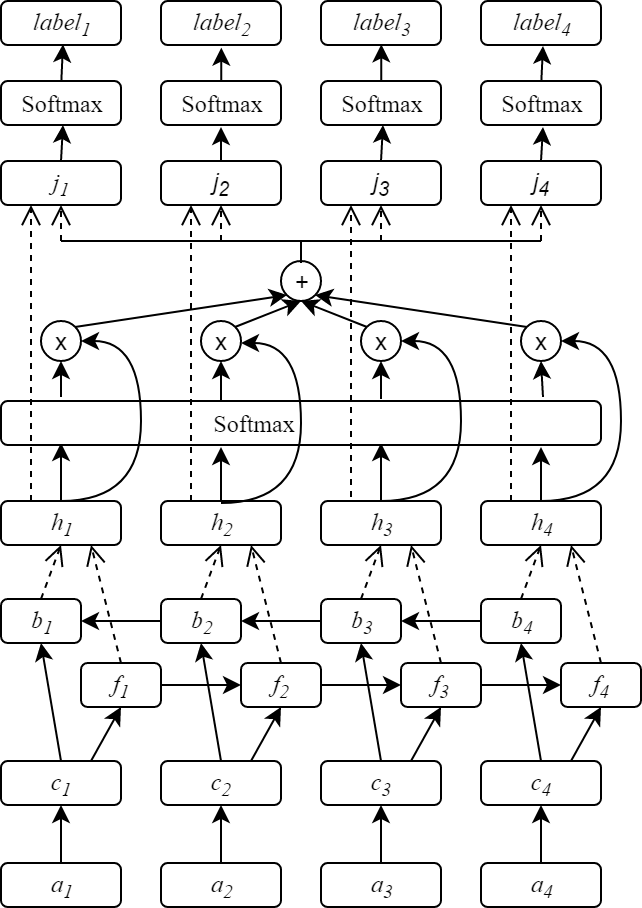
\includegraphics[width=3in]{cabilstm}
	\caption{An architecture of Context-Aware Bi-Directional Long Short Term Memories.}
	\label{fig:cabilstm}
\end{figure}

\section{Experiments}
In this chapter, we present our experiment results and the analysis accordingly. There are two set of scenarios. The first scenario set aims to find the best combination set of features. This scenario consists of four combinations as follows:

\begin{enumerate}
	\item Word Embedding (WE)
	\item Word Embedding + POS Tag (WE + POS)
	\item Word Embedding + Word Embedding of Neighbors (WE + WE-N)
	\item Word Embedding + POS Tag + Word Embedding of Neighbors (WE + POS + WE-N)
\end{enumerate}

The second scenario set evaluates two different architectures, which are the original BLSTM and CAB-BLSTM. Underlying both architectures is a Convolutional Neural Network (CNN) layer, in order to catch more information surrounding each time step. This second scenario also aims to see the effect of hyper-parameter tuning for the CAB-BLSTM.

\subsection{Evaluation Metrics}
As for evaluation, we use precision, recall and F1 metrics for all scenarios. The results are evaluated with partial match approach~\cite{seki2003probabilistic}.

\subsection{Feature Combination Scenario}
Table~\ref{tab:feature_scenario} shows the scenario results of four feature combinations. The highest result is achieved with combination of WE + POS, followed by WE + WE-N + POS, WE, and WE + WE-N, with F1 scores of 72.29\%, 72.22\%, 62.00\%, and 61.92\% respectively. From these results, we can see the big impact POS Tag contributes for the performance. Using POS Tag enhances the result up to 10.29\%, when we compare WE + POS and WE combinations. The explanation would be the fact that POS Tag contains meaningful information such as Noun and Adjective which describes the word, it thus supports the word embedding feature when the training data size is relatively low.

Surprisingly, when we combine the neighboring words of the argument as in WE + WE-N, the result slightly decreases by 0.08\%, compared to only using WE feature. This is also the case when we compare WE + WE-N with WE + WE-N + POS scenarios, which decreases by 0.07\% when we used neighboring words. It shows us that neighboring words do not improve the performance at all. We suggest that this is because the CNN layer already extracts these information implicitly, by capturing surrounding information and compressed it into one vector. Hence, we do not need explicit neighboring words as part of our features. 

\begin{table}
	\caption{Results of Feature Combination Scenario}
	\label{tab:feature_scenario}
	\begin{tabular}{llll}
		\toprule
		Features		&Precision	&Recall		&F1			\\
		\midrule
		WE				&	64.68\%				&	60.25\%				&	62.00\%	\\
		WE + POS		&	74.24\%				&	\textbf{71.26\%}	&	\textbf{72.29\%}	\\
		WE + WE-N		&	64.17\%				&	60.29\%				&	61.92\%	\\
		WE + POS + WE-N	&	\textbf{74.51\%}	&	70.69\%				&	72.23\%	\\
		\bottomrule
	\end{tabular}
\end{table}

Since WE + POS outputs the best result in terms of F1 score in this scenario set, we will use it for the next set of scenarios.

\subsection{Model Architecture Scenario}
The experiment results of the second scenario set are presented in Table~\ref{tab:architecture_scenario}. First we show the result using the original BLSTM with F1 score of 72.29\%. On the next experiment, we added the attention mechanism on top of the BLSTM layer, with three different dimensions $K$ of weight matrix $W \in {\rm I\!R^{H \times K}}$ from the Equation~\ref{sum_weight}. The three dimensions of $K$ are 64, 128, and 256. When we experimented on the first dimension size of $K$, 64, it is notable that the F1 score increases by 0.76\%. The performance keeps increasing as we add the dimension size of $K$ until 256 with F1 score of 74.78\% which increased by 2.49\% compared to the original BLSTM. We also obtained the highest precision and recall with dimension size $K$ of 256. However, when we added more dimension above 256, the model seems to be overfitting.

The results show that the CA-BLSTM architecture outperforms the original BLSTM architecture. We suggest that our proposed model can capture context information at abstract level. We believe that the attention mechanism plays an essential role to extract which word has the most significant value as a hint to predict the semantic roles of each time step.

\begin{table}
	\caption{Results of Model Architecture Scenario}
	\label{tab:architecture_scenario}
	\begin{tabular}{llll}
		\toprule
		Name			&Precision					&Recall		&F1			\\
		\midrule
		BLSTM				&	74.24\%				&	71.26\%				&	72.29\%	\\
		CA-BLSTM-64			&	73.37\%				&	73.25\%				&	73.05\%	\\
		CA-BLSTM-128		&	76.25\%				&	73.52\%				&	74.05\%	\\
		CA-BLSTM-256		&	\textbf{77.03\%}	&	\textbf{73.55\%}	&	\textbf{74.78\%}\\
		\bottomrule
	\end{tabular}
\end{table}


\section{Conclusions}
Semantic Role Labeling (SRL) is an integral part of understanding semantic information of a text. One of its applications is to make chat bots understand user's chat better and thus, it can provide more engaging answers. Even though the SRL on formal language has been widely studied, the conversational language used on chatting platform is barely tapped. In this work, we introduce a new set of semantic roles for conversational language and propose a new model architecture called Context-Aware Bi-Directional Long Short-Term Memories (CA-BLSTM). CA-BLSTM adds an attention mechanism on top of the BLSTM layer, by collecting context information from all the words in a sentence and representing it as a vector that is concatenated to all the output of BLSTM.

We conducted two set of experiment scenarios, which are evaluating feature combinations and architectures. Our experiments on feature combination show that when the size of training data is relatively small, one still needs to use traditional feature such as POS tag in addition to word embedding. For the experiment on architecture, the results show that our proposed architecture, CA-BLSTM, can outperforms the original BLSTM. Based on the increasing result of all precision, recall, and F1, we suggest that our architecture successfully extracts context information at higher level. Since it becomes more context-aware, our analysis shows that CA-BLSTM can predict the labels more carefully.

For future works, once the SRL system is establihed, one can focus on building the Natural Language Generation (NLG) system for chat bots based on the semantic roles of the conversational language. This way, we can create more intelligent chat bots which understand deeper on conversational language.

%\end{document}  % This is where a 'short' article might terminate
